\documentclass{scalatekids-article}
\usepackage[italian]{babel}
\begin{document}
\lfoot{Norme di Progetto 3.0.0}
\newgeometry{top=3.5cm}
\begin{titlepage}
  \begin{center}
    \begin{center}
      
\includegraphics[width=10cm]{sklogo.png}
    \end{center}
    \vspace{1cm}
    \begin{Huge}
      \begin{center}
        \textbf{Norme Di Progetto}
      \end{center}
    \end{Huge}
    \vspace{11pt}
    \bgroup\def\arraystretch{1.3}
    \begin{tabular}{r|l}
      \multicolumn{2}{c}{\textbf{Informazioni sul documento}}\\
      \hline
      \setbox0=\hbox{0.0.1\unskip}\ifdim\wd0=0pt
      \\
      \else
      \textbf{Versione} & 3.0.0\\
      \fi
      \textbf{Redazione} & \multiLineCell[t]{Andrea Giacomo Baldan\\Francesco Agostini\\Michael Munaro}\\
      \textbf{Verifica} & \multiLineCell[t]{Davide Trevisan\\Marco Boseggia\\Michael Munaro}\\
      \textbf{Approvazione} & \multiLineCell[t]{Giacomo Vanin}\\
      \textbf{Uso} & Interno\\
      \textbf{Lista di Distribuzione} & \multiLineCell[t]{ScalateKids}\\
    \end{tabular}
    \egroup
    \vspace{22pt}
  \end{center}
\end{titlepage}
\restoregeometry
\clearpage
\pagenumbering{Roman}
\setcounter{page}{1}
\begin{flushleft}
  \vspace{0cm}
  {\large\bfseries Diario delle modifiche \par}
\end{flushleft}
\vspace{0cm}
\begin{center}
  \begin{longtable}{| l | l | l | l | p{5cm} |}
    \hline
    Versione & Autore & Ruolo & Data & Descrizione \\
    \hline
    2.3.0 & & & 2016-05-06 & Verifica sezione Analisi Statica 5.4.1.1\\
    \hline
    2.2.0 & & & 2016-05-06 & Verifica sezione Progettazione Architetturale 2.2.3 e sottosezione Definizione di Prodotto 2.2.3.2.2\\
    \hline
    2.1.2 & & & 2016-05-05 & Incremento sezione Analisi Statica 5.4.1.1\\
    \hline
    2.1.1 & & & 2016-05-03 & Incremento sezione Progettazione Architetturale 2.2.3, sottosezione Definizione di Prodotto 2.2.3.2.2\\
    \hline
    2.1.0 & Andrea Giacomo Baldan & Verificatore & 2016-05-01 & Verifica sezione Assicurazione Qualità\\
    \hline
    2.0.3 & Marco Boseggia & Analista & 2016-04-26 & Incremento sezione Assicurazione Qualità \\
    \hline
    2.0.2 & Marco Boseggia & Analista & 2016-04-26 & Spostamento sezione Assicurazione Qualità \\
    \hline
    2.0.1 & Michael Munaro & Analista & 2016-04-26 & Integrazione appendice Redmine per calendario attività \\
    \hline
    2.0.0 & Giacomo Vanin & Responsabile & 2016-03-20 & Approvazione documento\\
    \hline
    1.6.0 & Marco Boseggia & Verificatore & 2016-03-13 & Verifica sezione test\\
    \hline
    1.5.1 & Francesco Agostini & Analista & 2016-03-12 & Incremento sezione test\\
    \hline
    1.5.0 & Davide Trevisan & Verificatore & 2016-03-12 & Verifica sezioni 2.2.3 e sottosezioni\\
    \hline
    1.4.1 & Michael Munaro & Analista & 2016-03-11 & Incremento sezione 2.2.3 e sottosezioni\\
    \hline
    1.4.0 & Davide Trevisan & Verificatore & 2016-03-11 & Verifica sezione norme per la progettazione (2.2.3 e sottosezioni)\\
    \hline
    1.3.1 & Michael Munaro & Analista & 2016-03-10 & Aggiunta sezione norme per la progettazione (2.2.3 e sottosezioni)\\
    \hline
    1.3.0 & Davide Trevisan & Verificatore & 2016-03-06 & Verifica ultime sezioni modificate (2.2.2.1 e 4.5.1.3)\\
    \hline
    1.2.2 & Andrea Giacomo Baldan & Analista & 2016-03-05 & Incremento sezione 2.2.2.1 (ScalateTrack)\\
    \hline
    1.2.1 & Andrea Giacomo Baldan & Analista & 2016-03-05 & Incremento sezione 4.5.1.3 (Script di utilità locale)\\
    \hline
    1.2.0 & Michael Munaro & Verificatore & 2016-03-03 & Verifica sezioni 3.2, 4 e appendice A \\
    \hline
    1.1.3 & Andrea Giacomo Baldan & Analista & 2016-03-01 & Incremento Appendice\\
    \hline
    1.1.2 & Andrea Giacomo Baldan & Analista & 2016-02-26 & Incremento sezione 3.2.1 Norme di Verifica\\
    \hline
    1.1.1 & Andrea Giacomo Baldan & Analista & 2016-02-26 & Stesura sezione 4 Processi Organizzativi\\
    \hline
    1.1.0 & Marco Boseggia & Verificatore & 2016-02-24 & Verifica sezioni 1, 2 e 3\\
    \hline
    1.0.3 & Andrea Giacomo Baldan & Analista & 2016-02-21 & Stesura sezione 3 Processi di Supporto\\
    \hline
    1.0.2 & Andrea Giacomo Baldan & Analista & 2016-02-21 & Stesura sezione 2 Processi Primari\\
    \hline
    1.0.1 & Andrea Giacomo & Analista & 2016-02-19 & Riorganizzazione generale dei contenuti\\
    \hline
    1.0.0 & Alberto De Agostini & Responsabile & 2015-12-23 & Approvazione documento\\
    \hline
    0.5.0 & Davide Trevisan & Verificatore & 2015-12-22 & Verifica sezione Processi di Sviluppo\\
    \hline
    0.4.0 & Marco Boseggia & Verificatore & 2015-12-22 & Verifica sezione Processi di Supporto\\
    \hline
    0.3.2 & Andrea Giacomo Baldan & Amministratore & 2015-12-22 & Correzione sezione Processi di Sviluppo\\
    \hline
    0.3.1 & Francesco Agostini & Amministratore & 2015-12-21 & Correzione sezione Processi di Supporto\\
    \hline
    0.3.0 & Marco Boseggia & Verificatore & 2015-12-20 & Verifica sezione Processi di Sviluppo\\
    \hline
    0.2.0 & Michael Munaro & Verificatore & 2015-12-20 & Verifica sezione Processi di Supporto\\
    \hline
    0.1.2 & Andrea Giacomo Baldan & Amministratore & 2015-12-18 & Stesura sezione Processi di Sviluppo\\
    \hline
    0.1.1 & Francesco Agostini & Amministratore & 2015-12-18 & Stesura sezione Processi di Supporto\\
    \hline
    0.1.0 & Giacomo Vanin & Verificatore & 2015-12-17 & Verifica sezione Processi Organizzativi\\
    \hline
    0.0.2 & Andrea Giacomo Baldan & Amministratore & 2015-12-17 & Stesura sezione Processi Organizzativi\\
    \hline
    0.0.1 & Andrea Giacomo Baldan & Amministratore & 2015-12-16 & Creazione scheletro del documento\\
    \hline
  \end{longtable}
\end{center}
\tableofcontents
\newpage
\pagenumbering{arabic}

\section{Sommario}

\subsection{Scopo del documento}

Le Norme di Progetto hanno l'obiettivo di fornire il metodo di lavoro, le
convenzioni e formalismi che i membri del gruppo devono adottare nell'attuazione
delle strategie scelte durante l'\gloss{attività} di progetto. \\
Tutti i componenti del gruppo sono tenuti a leggere il presente documento e a seguire
le regole contenute; esso verrà integrato ogni qualvolta si presenti la necessità di
chiarire dubbi o definire comportamenti da seguire in specifici scenari.

\prodPurpose{}
\glossExpl{}

\subsection{Riferimenti}

\subsubsection{Informativi}

\begin{itemize}
\item\textbf{Redmine:} \url{http://www.redmine.org/};
\item\textbf{Docker:} \url{https://www.docker.io/};
\item\textbf{Travis-ci:} \url{https://travis-ci.org/};
\item\textbf{Virtual Box:} \url{https://www.virtualbox.org/}.
\end{itemize}

\section{Processi Primari}

\subsection{Fornitura}

\subsubsection{Studio di Fattibilità}

Il primo compito degli \textit{Analisti} sarà di redigere uno studio comparativo
dei lati positivi e negativi dei capitolati pubblicati secondo le opinioni e i
confronti dei membri del gruppo, evidenziando in particolare le criticità che
hanno portato all'esclusione dei capitolati scartati e, dal lato opposto, i
fattori positivi che hanno colpito e influenzato maggiormente la decisione
finale sul capitolato.

\subsubsection{Pianificazione e preparazione dell'offerta}

Al fine dell'aggiudicazione dell'appalto sul capitolato scelto, sarà compito del
\textit{Responsabile} stendere un \textit{Piano di Progetto} con sistemi di
controllo e rendicontazione ben delineati. Dovrà inoltre includere un'accurata
analisi dei rischi corredata di contromisure e un preventivo che all'avanzare
del progetto si trasformerà in consuntivo.\\
Il documento presenterà infine un organigramma, utile a definire la struttura
e l'allocazione delle risorse e i ruoli di progetto.\\
I \gloss{diagrammi di Gantt} e \gloss{PERT} (Program Evaluation Review
Technique) saranno utilizzati per rappresentare graficamente l'allocazione nel
tempo e la durata dei compiti, evidenziando le dipendenze tra le attività ed
il loro impatto sull'intero progetto.\\
Vedi~\ref{sec:ServiziWeb} per la strumentazione utile allo scopo.

\subsection{Sviluppo}

Gli \textit{Analisti} analizzeranno i Requisiti di Sistema del prodotto da
sviluppare, da questi sarà possibile estrarre i requisiti software e stendere un'analisi dettagliata.

\subsubsection{Analisi dei Requisiti}

Dal capitolato e dall'\gloss{attività} di \gloss{brainstorming} effettuata
inizialmente, integrata con le riunioni esterne da effettuare con il
\textit{Proponente}, gli \textit{Analisti} dovranno stilare una lista di casi
d'uso ed estrarre i requisiti emergenti.\\
I requisiti software dovranno essere:
\begin{itemize}
\item precisi;
\item non ambigui;
\item completi;
\item testabili.
\end{itemize}
Essi saranno composti da una parte testuale che descrive il requisito ed un
modello semiformale per esprimerli, nel nostro caso il linguaggio \gloss{UML}
\textit{versione 1.0}. Ogni diagramma inserito nei documenti dovrà essere
etichettato secondo la seguente regola:
\begin{center}
  \verb=<Tipo><Id>=
\end{center}
Dove \verb=Tipo= può assumere le seguenti sigle:
\begin{itemize}
\item\textbf{UC:} diagramma di caso d'uso;
\item\textbf{CD:} diagramma di classe;
\item\textbf{OD:} diagramma degli oggetti;
\item\textbf{SD:} diagramma di sequenza;
\item\textbf{AD:} diagramma di \gloss{attività};
\item\textbf{PD:} diagramma dei \gloss{package}.
\end{itemize}
\verb=Id= è un numero crescente che identifica
univocamente il caso d'uso. Se un caso d'uso è derivato da un altro, il suo id
sarà preceduto dall'id del caso d'uso da cui deriva e separato da esso con un
punto.

\subsubsection{Casi d'uso e tracciamento dei requisiti}

\label{sec:front-end}

\paragraph{ScalateTrack}
\label{sec:scalatetrack}

Per facilitare la gestione dei casi d'uso e il tracciamento dei requisiti va
utilizzata un'applicazione web sviluppata per lo scopo appositamente dal
gruppo.\\Essa si interfaccia con un database relazionale residente sul server
privato del gruppo (vedi~\ref{sec:server}) e permette una visualizzazione chiara
dei requisiti, dei casi d'uso e delle componenti. Una volta completata la
procedura d'inserimento dei dati, previa verifica, è possibile esportare i
requisiti in formato \LaTeX\xspace ed eseguirne il tracciamento automatico
rispetto alle fonti e viceversa. Allo stesso modo è possibile esportare le
componenti ed eseguirne il tracciamento automatico rispetto ai requisiti
che soddisfano e viceversa.

\begin{figure}[H]
  \begin{subfigure}[H]{0.47\textwidth}
    \centering
    \includegraphics[width=0.8\textwidth]{AggiuntaRequisito.png}
    \caption{Creazione nuovo requisito}
  \end{subfigure}
  \qquad
  \begin{subfigure}[H]{0.47\textwidth}
    \centering
    \includegraphics[width=0.8\textwidth]{AggiuntaUseCase.png}
    \caption{Creazione nuovo caso d'uso}
  \end{subfigure}
\end{figure}

\paragraph{Casi d'uso}

Ogni caso d'uso dovrà presentare i seguenti campi:
\begin{itemize}
\item Codice identificativo nella forma \verb=<UC><Id>= con \verb=UC= = Use
  Case mentre \verb=Id= è un numero crescente che identifica univocamente il
  caso d'uso. Se un caso d'uso è derivato da un altro, il suo \verb=Id= sarà
  preceduto dall'\verb=Id= del caso d'uso da cui deriva e separato da esso con un
  punto.
\item Titolo;
\item Diagramma \gloss{UML};
\item Attori primari;
\item Attori secondari;
\item Scopo e descrizione;
\item Precondizione;
\item Postcondizione;
\item Flusso principale degli eventi;
\item Scenari alternativi.
\end{itemize}

\paragraph{Requisiti software}

\label{sec:adr}
I requisiti all'interno del documento \textit{Analisi dei Requisiti} seguiranno le seguenti regole:
\begin{center}
  \verb=<Importanza><Tipologia><Id>=
\end{center}
Di seguito sono elencati i possibili valori che ogni termine tra parentesi angolari può assumere:
\begin{itemize}
\item \textbf{Importanza}:
  \begin{itemize}
  \item \textbf{OB} indica un requisito obbligatorio;
  \item \textbf{DE} indica un requisito desiderabile;
  \item \textbf{OP} indica un requisito opzionale.
  \end{itemize}
\item \textbf{Tipologia}:
  \begin{itemize}
  \item \textbf{F} indica un requisito funzionale;
  \item \textbf{Q} indica un requisito di qualità;
  \item \textbf{T} indica un requisito tecnologico;
  \item \textbf{V} indica un requisito di vincolo.
  \end{itemize}
\item \textbf{Id}: è un numero crescente che identifica univocamente il
  requisito. Se un requisito è stato derivato da un altro, il suo id sarà
  preceduto dall'id del requisito da cui dipende e separato da esso con un
  punto.
\end{itemize}

\subsubsection{Progettazione architetturale}

La \textit{Progettazione} precede la produzione ed è l'\gloss{attività} che
passa dai requisiti del problema, estratti dagli \textit{Analisti} durante
l'\textbf{Analisi}, ad una soluzione del problema preposto a carico dei
\textbf{Progettisti}. Essa dovrà rispettare tutti i requisiti che il gruppo ha
concordato con il \textit{Committente}.\\

\paragraph{Specifica Tecnica}

Sarà compiti dei \textit{Progettisti} definire la struttura ad alto livello.\\
Vengono definite:
\begin{itemize}
\item Le componenti software, definite dalla struttura ad alto livello;
\item Le interfacce verso l'esterno e tra le componenti;
\item Classi, tecniche e design pattern per lo sviluppo;
\item I Requisiti Software diventano Requisiti Componenti più dettagliati.
\end{itemize}

Dalla specifica dei Requisiti delle Componenti deriveranno i test da attuare in
attività di verifica, come specificato in~\ref{sec:NormeDiVerifica};

% \paragraph{Stile di progettazione}

\subparagraph{Design Pattern}

L'\gloss{attività} di \textit{Progettazione} dovrà fare utilizzo di
\gloss{design pattern} globalmente affermati e dovrà giustificarne la
scelta.\\Dovranno inoltre essere rispettati al massimo i paradigmi di
\gloss{OOP} (programmazione orientata agli oggetti) del linguaggio
\gloss{Scala}, con eventuale utilizzo di costrutti \gloss{funzionali},
coerentemente con l'utilizzo delle librerie \textit{\gloss{Akka}}.

\subparagraph{Componenti software}

Le componenti software all'interno del documento \textit{Specifica Tecnica}
dovranno essere nominate elencando prima del nome della classe tutti i namespace
in cui essa è contenuta separati da una coppia di due punti.\\ Qui possiamo
vedere un esempio:
\begin{center} \verb=actorbase::cli::views::CommandLoop=
\end{center} Inoltre per facilitare la comprensione della lettura dei diagrammi
dei package e delle classi si è scelto di:
\begin{itemize}
\item usare una colorazione diversa per package di livelli diversi;
\item usare il colore verde per indicare classi o package esterni al sistema.
\end{itemize}


\subparagraph{Tracciamento componenti}

Il software ScalateTrack (\ref{sec:scalatetrack}) si occupa anche del
tracciamento dei componenti. Nello specifico ogni requisito può essere tracciato
con uno o più componenti, in questo modo il gruppo potrà controllare e garantire
che ogni requisito venga soddisfatto.\\ ScalateTrack inoltre genererà
automaticamente le tabelle dei tracciamenti requisiti-componenti e
componenti-requisiti.

\begin{figure}[H]
  \centering
  \includegraphics[width=0.2\textwidth]{AggiuntaComponente.png}
  \caption{Creazione nuovo componente}
\end{figure}

\subparagraph{Test di Integrazione}

I \textit{Progettisti} devono definire dei test necessari alla verifica del
corretto funzionamento delle componenti.

\subparagraph{Diagrammi UML}
\label{sec:diagrammiUmlSpecTec}
Nella specifica tecnica dovranno essere presentati diversi tipi di diagrammi, in
particolare i \textit{progettisti} avranno il compito di realizzare i seguenti
rispettando le regole imposte dallo standard \gloss{UML}
1.0:
\begin{itemize}
\item \gloss{diagrammi dei package};
\item \gloss{diagrammi delle classi};
\item \gloss{diagrammi di sequenza};
\item \gloss{diagrammi di attività}.
\end{itemize}

\paragraph{Definizione di prodotto}
I \textit{progettisti} oltre a redigere la \textit{Specifica Tecnica} avranno il
compito di produrre anche il documento \textit{Definizione di Prodotto} in cui
verrà descritta la progettazione di dettaglio del sistema andando ad analizzare
più in profondità l'architettura. Il livello di dettaglio sarà maggiore rispetto
alla \textit{Specifica Tecnica}, in particolare saranno definite le interazioni
tra le classi e la definizione degli attributi e dei metodi contenuti, in modo
da fornire ai programmatori un documento da seguire precisamente per la
creazione del prodotto.

\subparagraph{Definizione delle classi}
All'interno della \textit{Definizione di prodotto} dovrà essere descritta ogni
classe presente all'interno del sistema. Per ognuna di queste classi la descrizione
dovrà essere comprensiva di:
\begin{itemize}
\item Elenco dei metodi;
\item Elenco dei parametri;
\item Spiegazione dello scopo della classe;
\item Funzionalità che essa modella.
\end{itemize}

\subparagraph{Tracciamento classi}

In questo documento dovrà essere presente il tracciamento dei requisiti abbinato
alle classi che lo soddisfano.\\Come per la \textit{Specifica Tecnica} anche in
questo caso verrà utilizzato il software ScalateTrack (\ref{sec:scalatetrack})
il quale renderà automatico l'esportazione in formato \LaTeX\xspace delle
tabelle di tracciamento classi-requisiti e requisiti-classi.

\begin{figure}[H]
  \centering
  \includegraphics[width=0.2\textwidth]{RQ/TracciamentoClasses.png}
  \caption{Creazione nuova classe}
\end{figure}

\subparagraph{Diagrammi UML}

Dovranno essere aggiornati i seguenti diagrammi rispettando gli stessi standard
stabiliti per produrre la \textit{Specifica Tecnica} (\ref{sec:diagrammiUmlSpecTec}):
\begin{itemize}
\item \gloss{diagrammi delle classi};
\item \gloss{diagrammi di sequenza};
\item \gloss{diagrammi di attività}.
\end{itemize}

\section{Processi di Supporto}

\subsection{Documentazione}

\subsubsection{Struttura dei documenti}

\label{sec:strutturadoc}
Abbiamo standardizzato la scrittura di tutti i documenti attraverso un
\gloss{template} \LaTeX\xspace appositamente creato e presente su
\textit{\gloss{GitHub}} nel \gloss{repository} \textit{ActorBase-Documents}.\gloss{git} (vedi~\ref{sec:ServiziWeb}).\\
L'uso del \gloss{template} ci permette di creare una serie di documenti
stilisticamente uniformi tra loro e ci facilita la modifica delle parti in
comune tra essi.\\Facilita inoltre la creazione di nuove \gloss{macro} e comandi
\LaTeX\xspace. Nella fattispecie abbiamo creato i seguenti:
\begin{itemize}
\item\verb=\gloss=: Da utilizzare per inserire le parole da glossario;
\item\verb=\glossDef=: Da utilizzare all'interno del documento \textit{Glossario} per inserire nuove definizioni;
\item\verb=\glossaryLetter=: Da utilizzare all'interno del documento \textit{Glossario} per inserire le sezioni alfabetiche preformattate;
\item\verb=\prodPurpose=: Da utilizzare per creare la sottosezione ``Scopo del Prodotto'', da inserire nelle parti comuni di tutti i documenti (Sommario);
\item\verb=\glossExpl=: Da utilizzare per creare la sottosezione ``Glossario'', da inserire nelle parti comuni di tutti i documenti per spiegare come vengono identificati i termini da glossario;
\item\verb=\multiLineCell=: Da utilizzare per creare celle multilinea nelle tabelle.
\end{itemize}
Sono stati infine ridefiniti alcuni comportamenti dei comandi standard di
\LaTeX\xspace, per esempio le intestazioni e i piè pagina automatizzati, la
profondità delle \gloss{section}, dell'indice dei contenuti e le colorazioni dei
\gloss{link}:
\begin{itemize}
\item\textbf{\gloss{url}:} Blu;
\item\textbf{citazioni:} Grigio.
\end{itemize}
Riassumendo il \gloss{template} regola:
\begin{itemize}
\item Formattazione dei documenti (font);
\item Formattazione delle pagine (header e footer pagine);
\item Raggruppa tutti i pacchetti utilizzati;
\item Aggiunge comandi personalizzati;
\item Collegamenti tra indice e categorie o sezioni.
\end{itemize}
Ogni documento presenta in ordine:
\begin{itemize}
\item Logo del gruppo;
\item Informazioni del documento;
\item Diario delle modifiche: è una tabella in cui sono scritte le diverse modifiche fatte dai membri sul documento;
\item Indice: indice con collegamenti alle categorie e alle sezioni del documento;
\item Sommario: contiene alcune sottosezioni:
  \begin{itemize}
  \item Scopo del documento;
  \item Scopo del prodotto;
  \item Glossario;
  \item Riferimenti inerenti al documento in questione;
  \end{itemize}
\item Resto del documento: contenuto specifico.
\end{itemize}

\subsubsection{Struttura Pagina}

L'intestazione di ogni pagina contiene:
\begin{itemize}
\item Logo gruppo;
\item Nome gruppo;
\item Sezione corrente del documento.
\end{itemize}
Il piè pagina invece contiene:
\begin{itemize}
\item Nome documento;
\item Pagina corrente rispetto al numero di pagine totali.
\end{itemize}

\subsubsection{Norme tipografiche}

Per uniformare il più possibile la stesura di tutti i documenti queste sono le regole che tutto il gruppo deve seguire:

\paragraph{Punteggiatura}

\begin{itemize}
\item \textbf{Punteggiatura}: tutti i segni di punteggiatura devono essere seguiti da uno spazio e non avere spazi precedenti al segno stesso;
\item \textbf{Maiuscole}: le lettere maiuscole devono essere usate dove previsto dalla lingua italiana.
  Saranno inoltre scritti con l'iniziale maiuscola i ruoli, le persone inerenti al progetto e i documenti noti (es. \textit{Committente} \textit{Analisi dei Requisiti}). Gli acronimi saranno interamente scritti in maiuscolo (es. \textit{SQL}).
\end{itemize}

\paragraph{Stile testo}

\begin{itemize}
\item \textbf{Corsivo}: il corsivo dev'essere utilizzato per:
  \begin{itemize}
  \item Figure inerenti al progetto;
  \item Abbreviazioni;
  \item Citazioni;
  \item Documenti (es. \textit{Analisi dei Requisiti});
  \item Porre un'enfasi maggiore alla parola e/o frase;
  \end{itemize}
\item \textbf{Grassetto}: il grassetto dev'essere usato per:
  \begin{itemize}
  \item Evidenziare passaggi o concetti importanti;
  \item Sezioni e sottosezioni dei documenti;
  \end{itemize}
\item \textbf{Monospace}: i font monospace saranno usati per riportare parti di \gloss{codice}.
\end{itemize}

\paragraph{Formati di riferimento}

\begin{itemize}
\item \textbf{Riferimenti}:
  \begin{itemize}
  \item Percorsi web: per gli indirizzi web e per gli indirizzi e-mail deve essere usato il comando \LaTeX\xspace:
    \begin{center}
      \verb=\url{percorso}=
    \end{center}
  \item \gloss{Link} ad altri \gloss{PDF}:
    \begin{center}
      \verb=\href{run:<pathToPDF>/<namefile.pdf>}{<name of the link>}=
    \end{center}
  \item \gloss{Link} a sezioni interne al documento: per \gloss{link} a sezioni interne al documento corrente deve essere utilizzato il documento \LaTeX\xspace:
    \begin{center}
      \verb=\ref{riferimento a sezione}=
    \end{center}
  \end{itemize}
\item \textbf{Date}: Le date devono essere espresse seguendo lo standard \textit{\gloss{ISO}} 8601:2004:
  AAAA-MM-GG
  AAAA: rappresenta l'anno (es. 2015);
  MM: rappresenta il mese (es. 12);
  GG: rappresenta il giorno (es. 21).

\item \textbf{Abbreviazioni}: per semplicità possono essere abbreviati i nomi dei seguenti documenti:
  AR: \textit{Analisi dei Requisiti};
  RR: \textit{Revisione dei Requisiti};
  GL: \textit{Glossario};
  NP: \textit{Norme di Progetto};
  RP: \textit{Revisione di Progettazione};
  PQ: \textit{Piano di Qualifica};
  RQ: \textit{Revisione di Qualifica};
  PP: \textit{Piano di Progetto};
  SF: \textit{Studio di Fattibilità};
  RA: \textit{Revisione di Accettazione}.

\item \textbf{Nomi ricorrenti}:
  \begin{itemize}
  \item Ruoli: come già scritto in precedenza i ruoli di progetto devono essere scritti con la prima lettera di ogni parola maiuscola ed in corsivo, escludendo le proposizioni (es. \textit{Responsabile di Progetto});
  \item Nomi dei \gloss{file}: i nomi dei \gloss{file} relativi a documenti devono seguire;
    la notazione \textit{\gloss{UpperCamelCase}}, seguiti da \textit{\_v} e dalla
    versione del \gloss{file} (es. NormeDiProgetto\_v1.0.1.pdf);
  \item Nome del progetto: sarà indicato come \textbf{Actorbase};
  \item Nome del \textit{Committente}: il \textit{Committente} sarà indicato come \textit{prof. Tullio Vardanega};
  \item Nome del \textit{Proponente}: il \textit{Proponente} sarà indicato come \textit{prof. Riccardo Cardin};
  \item Nome del gruppo: il gruppo sarà indicato come \textit{ScalateKids}.
  \end{itemize}
\end{itemize}

\paragraph{Immagini}

Utilizziamo immagini con formato \textit{JPG} o \textit{PNG}, questi ultimi rendono immediata l'inclusione delle suddette immagini nei documenti.

\paragraph{Integrazione termini di lingua straniera}

Per non incorrere in diverse modalità di integrazione per l'uso di vari termini
di lingua straniera (es. \gloss{file}, \gloss{repository} etc.) i termini non italiani non saranno pluralizzati, esempio:\\
\begin{center}
  \verb=abbiamo utilizzato dei= \textit{repository} \verb=per... (non= \textit{repositories}\verb=)=.
\end{center}
Questa scelta è derivata da una ricerca che ha fornito diverse fonti riguardanti l'uso di questa norma nella lingua italiana, il sottostante sito web ne raccoglie buona parte:\\
\begin{center}
  \url{http://www.darsch.it/?pg=sphere&postid=954}
\end{center}

\subsubsection{Versionamento documenti}

La documentazione prodotta deve avere un numero di versione avente la seguente struttura:\\
\begin{center}
  vX.Y.Z
\end{center}
in cui:
\begin{itemize}
\item \textbf{X}: aumenta  ad ogni approvazione effettuata dal \textit{Responsabile}. Questo valore corrisponderà anche con il numero di uscite formali del documento:
  \begin{enumerate}
  \item\gloss{Attività} di \textbf{Analisi} che si conclude con la \textbf{RR};
  \item\gloss{Attività} di \textbf{Analisi di Dettaglio} che si conclude con l'ingresso alla \textbf{RP};
  \item\gloss{Attività} di \textbf{Progettazione Architetturale} che si conclude con la \textbf{RP};
  \item\gloss{Attività} di \textbf{Progettazione di Dettaglio e Codifica} che si conclude con l'ingresso alla \textbf{RQ};
  \item\gloss{Attività} di \textbf{Verifica e Validazione} che si conclude con la \textbf{RA}.
  \end{enumerate}
\item \textbf{Y}: aumenta ad ogni \gloss{attività} di verifica applicata sul documento. Quando il documento viene approvato dal \textit{Responsabile} questo numero viene azzerato;
\item \textbf{Z}: aumenta ad ogni modifica rilevante effettuata sul documento. Questo valore si azzera ad ogni \gloss{attività} di verifica o approvazione del documento.
\end{itemize}
La citazione di una versione specifica di un documento deve comprendere sia il nome che il numero di versione aderente al formato:
\begin{center}
  \textit{NomeDocumento\_vX.Y.Z}
\end{center}

\subsubsection{Ciclo di vita dei documenti}

Tutti i documenti nascono nello stato di \textit{in lavorazione}.\\
Dopo l'avvenuta di tutte le modifiche necessarie per arrivare ad una versione completa del documento, il suddetto si verrà a trovare nello stato \textit{da verificare}.\\
Alla fine della fase di verifica del documento, se approvato, il documento andrà nello stato di \textit{approvato}.
I tre stati sono descritti brevemente come segue:
\begin{itemize}
\item \textbf{In lavorazione}: il documento nasce in questo stato e ci rimane fino a che non è avvenuta una sua completa stesura;
\item \textbf{Da verificare}: il documento resta in questo stato finché i \textit{Verificatori} assegnati ad esso non effettueranno un controllo atto a trovare e a correggere errori di ogni tipo;
\item \textbf{Approvato}: dopo la fase di verifica il \textit{Responsabile} effettuerà una fase di approvazione, se questa fase sarà superata il documento sarà approvato e entrerà in una versione ufficiale.
\end{itemize}

\subsubsection{Norme di codifica dei file}

Tutti i \gloss{file} contenenti \gloss{codice} o documentazione dovranno essere conformi alla
codifica \gloss{UTF-8}.

\paragraph{Linee guida stilistiche}

La stesura del \gloss{codice} dovrà seguire pedissequamente alcune regole al fine di
garantire un buon livello di manutenibilità e verificabilità del prodotto, in
particolare gli sviluppatori dovranno attenersi alla \textit{Scala Style Guide}
(\url{https://docs.scala-lang.org/style/}), in particolar modo non possono
essere infrante le seguenti regole:
\begin{itemize}
\item Lunghezza massima linee 80 caratteri;
\item Indentazione di 2 spazi;
\item Posizionamento di parentesi graffe in linea con il blocco struttura di
  riferimento.
\end{itemize}
Tutti i \gloss{file} contenenti \gloss{codice} dovranno essere redatti in lingua inglese.

\subparagraph{Nomenclatura}

I nomi di variabili, metodi e funzioni seguiranno la convenzione
\textit{\gloss{lowerCamelCase}}, i nomi di classi invece seguiranno la
convenzione \textit{\gloss{UpperCamelCase}}.

\subparagraph{Ricorsione}

Il paradigma funzionale incentiva all'uso di ricorsione piuttosto che cicli
iterativi, è ammesso dunque l'utilizzo di ricorsione purchè si tratti
specificamente di ricorsione in coda, questo perchè in \gloss{Scala} tal
costrutto è ottimizzato in modo da non rimpeire lo \gloss{stack} assegnato alla
funzione chiamante. La ricorsione non in coda va invece evitata il più
possibile. Per ogni funzione ricorsiva sarà necessario fornire una prova di
terminazione. L'utilizzo deve giustificare la spesa in termini di memoria
rispetto al risparmio in termini di istruzioni.

\subparagraph{Documentazione}

I \gloss{file} contenenti \gloss{codice} dovranno essere adeguatamente commentati seguendo le
linee guida \gloss{scaladoc} \url{https://docs.scala-lang.org/style/scaladoc.html} ed essere provvisti di un
intestazione contenente:
\begin{lstlisting}
  /**
  * Licenza MIT
  * Nome file
  * Breve descrizione
  *
  * @author Autore del file
  * @version Versione
  * @date Data di creazione
  * Descrizione dettagliata del file
  */
\end{lstlisting}
Prima di ogni metodo dovrà essere presente un commento \gloss{scaladoc} contenente:
\begin{lstlisting}
  /**
  * Breve descrizione del metodo
  *
  * @param Nome del primo parametro
  * @param Nome del secondo parametro
  * @return Valore di ritorno del metodo
  * @throws Eccezioni lanciate dal metodo
  */
\end{lstlisting}
La documentazione verrà generata da \gloss{scaladoc}. Nel caso si verifichi la
necessità di documentare del \gloss{codice} di difficile comprensione, sarà possibile
inserire un commento nelle righe precedenti, dopo aver verificato
l'impossibilità di effettuare un \gloss{refactoring}.

\subsubsection{Glossario}

Il glossario è un documento unico per tutti i documenti, esso conterrà tutte le
definizioni, in ordine lessicografico crescente dei termini inerenti al tema
del progetto o che possono essere fraintesi. I termini che dovranno essere
inseriti nel glossario saranno contrassegnati da una \textit{G} pedice
all'interno dei documenti. Prima di inserire un nuovo termine bisognerà
assicurarsi che non sia già presente.\\ Il comando \LaTeX\xspace da utilizzare
per contrassegnare un termine da glossario all'interno dei documenti è
\verb=\gloss=, mentre l'inserimento di una nuova parola all'interno del
glossario è \verb=\glossDef= (come specificato in~\ref{sec:strutturadoc}). La
scelta di creare un comando apposito per un'operazione ``elementare'' è
scaturita dall'agevolazione che porta alla stesura della documentazione: avendo
un modo univoco di riconoscere i termini all'interno del glossario, è possibile
automatizzare il controllo delle parole da glossario all'interno dei
documenti (vedi sezione~\ref{sec:script}).

\section{Processi Organizzativi}

\subsection{Ruoli di progetto}

Durante l'intera \gloss{attività} di sviluppo del progetto, dalla formazione del gruppo alla
\textit{Revisione di Accettazione}, vi saranno alcuni ruoli ben precisi da ricoprire. Si
tratta di funzioni aziendali assegnate al progetto, specializzate in campi ben
specifici all'interno dell'azienda. Tra questi ruoli alcuni avranno maggior
presenza in determinate fasi rispetto ad altre, dove addirittura
potrebbero non figurare completamente, ma tutti sono essenziali per il buon
esito del progetto.\\ Ciascun componente dovrà ricoprire almeno una volta ogni
ruolo. Sarà inoltre possibile ricoprire più ruoli, sia contemporaneamente che in
distinte fasi del progetto, purché sia garantita l'assenza di conflitti
d'interesse nello svolgimento di \gloss{attività} di verifica e approvazione.\\
Al fine di garantire che tutti i componenti ricoprano tutti i ruoli almeno una volta, il gruppo seguirà le seguenti regole:
\begin{itemize}
\item Ogni componente non deve impiegare più del 50\% delle ore di lavoro in un unico ruolo;
\item Tutti i ruoli eccetto \textit{Responsabile di Progetto} e \textit{Amministratore} dovranno ruotare ogni due settimane;
\item I ruoli \textit{Responsabile di Progetto} e \textit{Amministratore} dovranno ruotare ogni venti giorni.
\end{itemize}
La scelta di ruotare con maggiore frequenza i ruoli al di fuori del
\textit{Responsabile} e \textit{Amministratore} è dettata essenzialmente dalla
maggiore cardinalità degli altri ruoli all'interno del gruppo, e
all'accentramento di responsabilità che \textit{Responsabile} e
\textit{Amministratore} comprendono naturalmente da contratto.

\subsubsection{Responsabile di Progetto}

Il \textit{Responsabile di Progetto} rappresenta il gruppo presso il \textit{Proponente}
e presso il \textit{Committente}. È il ruolo più presente lungo tutto l'arco temporale di
sviluppo del prodotto, in quanto deve partecipare e seguire il prodotto dalla
crescita fino al rilascio. Deve avere conoscenze e capacità
tecniche tali da comprendere e anticipare l'evoluzione del progetto.\\
Detiene il potere decisionale e ha responsabilità su:
\begin{itemize}
\item Pianificazione;
\item Gestione delle risorse umane;
\item Controllo, coordinamento e relazioni esterne;
\item Analisi e gestione dei rischi;
\item Approvazione dei documenti;
\item Approvazione dell'offerta economica.
\end{itemize}
Si occupa dunque della distribuzione delle \gloss{attività}, verifica che esse vengano
portate a termine seguendo le \textit{Norme di Progetto} e controlla che non vi
siano conflitti d'interesse tra redazione e verifica, ha il compito inoltre di
risolvere eventuali situazioni critiche tra i componenti del gruppo qualora
sorgessero conflitti.\\ Redige il \textit{Piano di Progetto} e collabora alla
stesura del \textit{Piano di Qualifica}.

\subsubsection{Analista}

L'\textit{Analista} è una figura molto presente nelle prime fasi del progetto e
determina fortemente la buona riuscita del prodotto. Non si occupa della
soluzione al problema ma deve offrire una specifica di progetto che comprenda
appieno la natura e la complessità del problema, che possa essere in seguito
valutata dal \textit{Progettista} al fine di fornire una soluzione.\\ Redige lo
\textit{Studio di Fattibilità} e l'\textit{Analisi dei Requisiti}, partecipa
inoltre alla stesura del \textit{Piano di Qualifica}.
\subsubsection{Amministratore}
L'\textit{Amministratore} si occupa di allestire, seguire e migliorare
l'ambiente di lavoro, le responsabilità principali sono:
\begin{itemize}
\item Amministrazione delle risorse e delle infrastrutture;
\item Risoluzione di problemi legati alla gestione dei processi;
\item Gestione della documentazione di progetto;
\item Controllo di versioni e configurazioni;
\item Ricerca di strumenti che possano automatizzare compiti tediosi;
\item Ricerca di strumenti che possano semplificare il lavoro di verifica.
\end{itemize}
Redige le \textit{Norme di Progetto} e partecipa alla stesura del \textit{Piano
  di Qualifica}.

\subsubsection{Progettista}

Il \textit{Progettista} è una figura molto legata all'\textit{Analista}, in
quanto è responsabile delle \gloss{attività} di progettazione, si occupa dunque di
trovare una soluzione efficace al problema, sfruttando le proprie competenze
tecniche e tecnologiche sempre aggiornate. Si tratta di un ruolo generalmente
presente dalla fase di progettazione fino alla fine del progetto.
\subsubsection{Programmatore}
È responsabile delle \gloss{attività} di codifica e manutenzione del prodotto, gestisce
inoltre le componenti di ausilio necessarie all'\gloss{attività} di verifica e
validazione. Ha competenze tecniche specializzate, ricopre principalmente
le seguenti responsabilità:
\begin{itemize}
\item Implementazione delle soluzioni descritte dal \textit{Progettista}
  seguendone i design pattern proposti;
\item Documentare e commentare il \gloss{codice} in modo da renderlo più facilmente
  mantenibile;
\item Implementare dei test utili in fase di verifica e validazione.
\end{itemize}
Si occupa della redazione del \textit{Manuale Utente}.

\subsubsection{Verificatore}

La figura del \textit{Verificatore} partecipa alla realizzazione del prodotto per
tutta la durata assieme al \textit{Responsabile}, possiede grandi capacità di
giudizio e competenza tecnica, influenza molto fortemente l'aspetto qualitativo
del prodotto.\\ Ricopre le seguenti responsabilità:
\begin{itemize}
\item Si assicura che le \gloss{attività} seguano le direttive stabilite nelle \textit{Norme di Progetto};
\item Controlla la conformità di ogni stadio del ciclo di vita del prodotto.
\end{itemize}
Si occupa della redazione del \textit{Piano di Qualifica}.

\subsection{Comunicazioni}

\subsubsection{Comunicazioni esterne}

Per le comunicazioni esterne è stata creata una apposita casella di posta elettronica:
\begin{center}
  \verb=scalatekids@gmail.com=
\end{center}
Questa casella e-mail viene gestita dal \textit{Responsabile di Progetto} che è
colui che si occupa di comunicare con il \textit{Committente} del progetto o con
qualsiasi altra persona esterna al gruppo di lavoro. È stata impostata per
effettuare l'inoltro automatico delle mail in entrata verso gli indirizzi
di tutti i componenti del gruppo, in modo tale che ognuno possa ricevere una
copia della posta in ingresso. Soltanto il \textit{Responsabile} ha il
potere di inviare posta in uscita.

\subsubsection{Comunicazioni interne}

\label{sec:ComunicazioniInterne}
Per le comunicazioni interne verrà utilizzato un \gloss{forum} apposito su
\textit{Redmine} (vedi sezione~\ref{sec:redmine}), suddiviso in quattro sezioni
principali corrispondenti alle revisioni di avanzamento del progetto:
\begin{itemize}
\item Revisione dei Requisiti;
\item Revisione di Progettazione;
\item Revisione di Qualifica;
\item Revisione di Accettazione.
\end{itemize}
Ogni sezione è composta da due sottosezioni, riunioni e comunicazioni, le quali
conterranno rispettivamente le riunioni indette seguite dalla disponibilità dei
membri a partecipare e, a seguito di avvenuta riunione, il riassunto dei punti
discussi e le comunicazioni di carattere più o meno generale riguardanti
\gloss{attività} della revisione di appartenenza.\\ Ogni \gloss{topic} all'interno di
queste due sottosezioni dovrà rispettare il seguente formato:
\begin{itemize}
\item\textbf{Riunioni:}\\
  \textit{Riunione Dominio\ -\ Data AAAA-mm-dd\ -\ Oggetto}\\
  (es: Riunione Interna - 2015-12-29 - Strategie Ciclo di Vita)
\item\textbf{Comunicazioni:}\\
  \textit{Oggetto\ -\ Data}\\
  (es: Design Pattern - 2016-01-12)
\end{itemize}
La voce \textit{Oggetto} dovrà essere esplicativa del contenuto, il più
possibile stringata e non confondibile con precedenti \gloss{topic}. È ammesso
l'inserimento di allegati purché strettamente pertinenti al \gloss{topic}, ad
esempio il verbale di una riunione o il riassunto di discussioni avvenute al di
fuori delle riunioni.\\ Vengono usati altri strumenti ufficiosi per lo scambio
di informazioni:
\begin{itemize}
\item applicazioni di \gloss{instant messaging} quali \textit{Telegram} e il suo servizio \textit{Telegram Web};
\item applicazioni \gloss{VoIP} per effettuare audio conferenze con un qualsiasi numero di componenti, quale \textit{TeamSpeak3};
\item servizi online per la gestione di una \gloss{whiteboard} condivisa, quale \textit{Twiddla}.
\end{itemize}
Qualora membri del gruppo si scambino informazioni attraverso questi strumenti
sopra elencati dovranno, se presenti informazioni di interesse per il progetto,
mandare un sunto della suddetta conversazione sul \gloss{forum} per tenere
informati tutti i membri del gruppo sullo stato di avanzamento nella
sottosezione comunicazioni.\\ Solo in caso di necessità derivante dalla mancanza
di infrastrutture (es\. collegamento a internet) si potrà comunicare attraverso
SMS o chiamate telefoniche; anche in questo caso si dovrà verbalizzare quanto
detto attraverso il \gloss{forum} appena possibile.

\subsection{Riunioni}

\subsubsection{Riunioni Interne}

Tutti i componenti del gruppo possono avanzare una richiesta per una riunione
interna seguendo le regole apposite (vedi~\ref{sec:RegoleRichiesta}).\\
Sarà il \textit{Responsabile di Progetto} a decidere se indire
o meno la riunione proposta, controllando la disponibilità dei membri attraverso il
\gloss{forum} e, in caso, avvertendo tutti i componenti tramite un \gloss{topic} come
spiegato in sezione~\ref{sec:ComunicazioniInterne}.\\ È richiesta la partecipazione di
almeno quattro membri del gruppo. In casi particolari, come riunioni che
trattano specifici ambiti non di interesse collettivo o per l'avvicinarsi
a date di rilevante importanza, è possibile indire una riunione di gruppo con meno componenti
presenti, sempre previa approvazione del \textit{Responsabile}.

\subsubsection{Riunioni esterne}

Le riunioni esterne (incontri col \textit{Committente} o \textit{Proponente}) possono essere
proposte da qualunque membro del gruppo. Spetta sempre al \textit{Responsabile
  di Progetto} la decisione finale.\\ È necessaria la presenza di almeno il
50\% + 1 dei componenti.

\subsubsection{Regole per la richiesta}

\label{sec:RegoleRichiesta}
Le richieste vanno effettuate tramite mail al \textit{Responsabile} e devono avere come oggetto:
\begin{center}
  \verb=Richiesta riunione <tipo riunione>=
\end{center}
\verb=tipo riunione= può essere interna o esterna.
Il corpo della mail dovrà avere una struttura del tipo:
\begin{center}
  \verb=Motivazione: <motivo riunione>=
  \verb=Data proposta: <data>=
  \verb=Luogo proposto: <luogo>=
\end{center}

\subsubsection{Esiti Riunioni}

Ad ogni riunione verrà affidato il compito a uno dei presenti di verbalizzare un riassunto sugli argomenti trattati e i chiarimenti emersi durante tale riunione.\\
Il redattore del verbale avrà poi l'obbligo di condividerlo con tutti sul \gloss{forum} del gruppo.

\subsection{Infrastruttura}

\subsubsection{Apparato di collaborazione}

Per coordinare il lavoro tra i componenti del gruppo, trovandosi spesso a dover
operare in remoto, il gruppo ha scelto di utilizzare quanto più possibile gli
strumenti di condivisione e \gloss{versionamento} erogati come servizi web,
centralizzando gli strumenti organizzativi su server privato.

\paragraph{Servizi web}

\label{sec:ServiziWeb}
I servizi web utilizzati sono:
\begin{itemize}
\item\textbf{Google Drive:} è usato per lo scambio di \gloss{file} e documenti all'interno del gruppo, principalmente per \gloss{file} che non necessitano di \gloss{versionamento}.\\
  Questo spazio del gruppo è suddiviso in diverse cartelle per una migliore gestione e per facilitare la ricerca all'interno di esso;\\
  Il \textit{Responsabile di Progetto} ha il potere amministrativo dell'\gloss{account} in questione, quindi sarà quest'ultima persona ad occuparsi di garantire i giusti diritti ai membri del gruppo.
\item\textbf{GitHub:} per tutti i \gloss{file} che necessitano un sistema di \gloss{versionamento} viene usato il servizio offerto da \textit{GitHub}, l'indirizzo web del gruppo è:\\
  \begin{center}
    \url{https://github.com/scalatekids}
  \end{center}
\item\textbf{Twiddla:} è un sistema che offre una lavagna online condivisa, questo servizio è utilizzato dai membri del gruppo per discutere e lavorare assieme da remoto, utile all'\gloss{attività} di \gloss{brainstorming} e \textbf{Analisi};
\item\textbf{Gantter for Google Drive:} è uno strumento gratuito per la creazione di \gloss{diagrammi di Gantt}, utile alla creazione dei Gantt preventivi;
\item\textbf{Lucidchart:} piattaforma comprensiva di un piano di utilizzo
  gratuito per studenti, utile per la produzione dei diagrammi
  \gloss{UML} permettendo la collaborazione tra i componenti online.
\end{itemize}

\subsubsection{Server dedicato}

\label{sec:server}
Sono state installate alcune applicazioni per il coordinamento del gruppo su
server dedicato, gestito dall'\textit{Amministratore} su direttive del
\textit{Responsabile}.\\ Il server è raggiungibile da interfaccia web previo
login, i componenti possono usufruire delle seguenti applicazioni:

\paragraph{Redmine}

Redmine è un'applicazione web atta alla gestione di progetti.\\
Offre diverse funzionalità che il gruppo dovrà utilizzare, quali:
\begin{itemize}
\item\textbf{Sezione wiki:} una pagina web in cui il gruppo andrà a condividere una serie di \gloss{link} di interesse riguardanti ogni tecnologia o aspetto inerente al progetto.
\item\textbf{Sistema di segnalazioni:} un sistema di segnalazioni gestite dall'\textit{Responsabile}, ogni segnalazione rappresenta un \gloss{task} assegnato ad uno o più membri del gruppo, il suo conseguimento servirà per il soddisfacimento di un requisito.
\item\textbf{Gantt:} \textit{Redmine} costruisce automaticamente un \gloss{diagramma di Gantt} con le segnalazioni create dall'\textit{Responsabile}
\end{itemize}
Per maggiori esplicazioni sull'utilizzo è stata redatta una sezione apposita~\ref{sec:redmine}.

\paragraph{PHPMyAdmin}

\textit{PHPMyAdmin} è uno strumento scritto in linguaggio \textit{PHP} che offre una facile amministrazione di \textit{\gloss{database}}.\\
Questo strumento verrà usato per la creazione di un back-end per la gestione dei requisiti.\\
Per la gestione e il tracciamento dei requisiti è stata creata un'interfaccia protetta da login (vedi sezione~\ref{sec:front-end}).

\subsubsection{Versionamento}

Lo strumento scelto è \gloss{git}, principalmente per la grande diffusione negli
ambienti di sviluppo e per l'integrazione offerta dal servizio web
\textit{GitHub}. Esso offre, inoltre, un'esaustiva documentazione
sull'utilizzo del programma in questione. Infine \gloss{git} si è rivelato essere
il più conosciuto tra i membri del gruppo. L'alternativa \gloss{SVN}, nonostante
i simili principi di funzionamento, costituiva una scelta più difficoltosa, in
quanto nessun membro ha mai avuto esperienze di utilizzo passate.

\paragraph{Repository}

Sono stati creati due \gloss{repository} all'indirizzo \url{https://github.com/scalatekids}:
\begin{itemize}
\item Actorbase.\gloss{git}: Conterrà i sorgenti del software vero e proprio;
\item Actorbase-Documents.\gloss{git}: Conterrà i sorgenti \LaTeX\xspace e i \gloss{PDF} generati;
\item Actorbase-Docker.\gloss{git}: Conterrà i sorgenti delle immagini
  \gloss{Docker} e i sorgenti dei test di unità da inserire di volta in volta.
  Si suddivide in:
  \begin{itemize}
  \item Actorbase-Docker/Latex.\gloss{git}: Conterrà il \gloss{Dockerfile}
    istruito per la creazione di un'immagine \textit{Ubuntu:Trusty} fornita
    dei pacchetti latex essenziali alla stesura dei documenti, corredata da
    \gloss{script} di generazione, verifica ortografica e leggibilità dei
    \gloss{PDF} generati.
  \item Actorbase-Docker/Scala.\gloss{git}: Conterrà il \gloss{Dockerfile}
    istruito per la creazione di un'immagine \textit{Ubuntu:Trusty} fornita
    di \textit{JVM v8} e \gloss{sbt}, corredata dai test di unità e
    \gloss{script} di analisi statica e qualitativa del \gloss{codice}.
  \end{itemize}
\end{itemize}
I \gloss{branch} dovranno essere nominati completamente in minuscolo, in lingua
inglese ed essere esplicativi del loro utilizzo.

\subsection{Integrazione continua}

Fin da subito, i \gloss{repository} saranno collegati ad un sistema di
\gloss{integrazione continua}, la scelta è ricaduta su \textit{Travis-CI} per la
semplicità di utilizzo e modeste esperienze passate di alcuni componenti del
gruppo.

\paragraph{Travis-CI}
\label{sec:travis}

È un servizio di \gloss{integrazione continua} comprensivo di un piano di
utilizzo gratuito. Facilmente configurabile, il collegamento ai \gloss{repository}
\textit{GitHub} avviene mediante un \gloss{file} di configurazione chiamato \textit{.travis.yml}
da inserire all'interno del \gloss{repository}. È inoltre possibile fornire
direttive al servizio e automatizzare unità di test su tutti i \gloss{file} del
\gloss{repository}, le quali possono essere lanciate sia dopo ogni \gloss{push}
che dopo ogni \gloss{pull} e notificare il \textit{Responsabile} via mail su
eventuali \gloss{commit} che non superino i test predisposti o violino
determinate regole.

\paragraph{Docker}

Dopo varie ricerche, \textit{\gloss{Docker} versione 1.9.1} è stato adottato per uniformare quanto più
possibile l'ambiente di test, grazie al sistema di \gloss{containerizzazione} e
\gloss{versionamento} delle immagini virtuali che offre.\\ Mediante un \gloss{file} di
configurazione principale, il \gloss{Dockerfile}, è possibile istruire il
programma e generare una o più immagini virtuali fornite dei soli pacchetti o
\gloss{script} necessari al testing a cui saranno adibite. Utilizzato in coppia con
\textit{Travis-CI} permette di effettuare test molto precisi e, allo stesso
tempo, di versionare un gran numero di immagini virtuali per diversificare i test e
gli ambienti su cui lanciarli. I \gloss{Dockerfile} infatti possono essere
versionati mediante un \gloss{repository} \textit{GitHub} direttamente collegato a
\textit{Travis-CI}, il quale, istruito ad hoc, si occuperà di generare
l'immagine \gloss{Docker} e caricarla mediante un \gloss{push} sull'\gloss{hub}
\gloss{Docker} presente nel sito \url{hub.docker.com}.\\ In questo modo i test
potranno essere versionati di pari passo con l'\gloss{attività} di sviluppo, garantendo
un accurata \gloss{attività} di verifica sui sorgenti e documenti senza gravare in alcun
modo sull'ambiente di lavoro di ogni singolo membro.
\begin{figure}[H]
  \centering
  \includegraphics[width=0.7\textwidth,keepaspectratio]{Docker.png}
  \caption{Integrazione continua\ -\ Travis-CI + Docker}
\end{figure}
Attualmente è in uso l'immagine \verb=scalatekids-latex= per la verifica dei documenti.

\subsubsection{Ambiente di lavoro individuale}

Per il lavoro individuale, è stato pensato ad un modo di uniformare quanto più
possibile l'ambiente di sviluppo tra i componenti; il \textit{Responsabile} e
l'\textit{Amministratore} hanno stabilito il sistema operativo e l'\gloss{IDE} di base ed è stata creato
un ambiente virtuale comune utilizzando il software \textit{Virtualbox versione 5.0.12} o superiore. Il sistema scelto è \textit{Ubuntu 14.04}.
Tutti i componenti del gruppo utilizzeranno gli strumenti all'interno della
\gloss{virtual machine} in modo da garantire omogeneità, e riproducibilità di
eventuali \gloss{bug}.\\ L'\textit{IDE} scelto è \textit{IntelliJIdea}, considerato il
più appropriato e compatibile con le tecnologie centrali del progetto. Gli
editor \textit{vim}, \textit{emacs} o \textit{Sublime Text 2} potranno essere
utilizzati dai componenti del gruppo, purché si tratti di modifiche rapide o
stesura di \gloss{script} di utilità generale.\\
Per la stesura dei documenti, l'\gloss{IDE} di riferimento è \textit{TeXstudio}.

\paragraph{Installazione virtual machine}

\label{sec:MacchinaVirtuale}
Una volta ottenuto il \gloss{file} \textit{.vdi} presente sul \gloss{\textit{Drive}} del gruppo
in forma compattata \textit{.7z}, ogni componente dovrà installare il software
\textit{Virtualbox} sul proprio computer e procedere con la creazione della
macchina virtuale.\\
I passi da seguire sono:
\begin{itemize}
\item Nuovo;
\item Tipo: \textit{Ubuntu} Versione: \textit{64-bit};
\item Assegnare la quantità di memoria in base alla propria disponibilità;
\item Usa un hard-disk esistente e selezionare \textit{ScalateKids-VMvX.Y.vdi}.
\end{itemize}
Una volta avviata la macchina, da terminale lanciare il comando:
\begin{center}
  \verb=curl http://codep.kissr.com/sk/scripts/init.sh | sh=
\end{center}
Il comando provvederà al download delle librerie e degli \gloss{script}
necessari alla corretta configurazione dell'ambiente di lavoro del gruppo.
Al termine la macchina virtuale sarà pronta ad essere utilizzata per lo sviluppo.

\paragraph{Versionamento virtual machine}

Di volta in volta, lungo tutto l'arco del progetto, quando sarà necessario
modificare l'ambiente di lavoro o ci sarà bisogno di librerie di supporto
ulteriori o modifica di \gloss{script} di utilità, il seguente comando si
occuperà di scaricare e installare gli aggiornamenti richiesti:
\begin{center}
  \verb=curl http://codep.kissr.com/sk/scripts/update.sh | sh=
\end{center}
Gli \gloss{script} di utilità citati comprenderanno strumenti di verifica e
leggibilità dei documenti.\verb=Init.sh= e \verb=update.sh=,
presenti sul server privato, saranno preparati dall'\textit{Amministratore} e
rilasciati di volta in volta previa approvazione del \textit{Responsabile}.

\paragraph{Script di utilità locali}

\label{sec:script}
L'\textit{Amministratore} si è occupato di scrivere alcuni \gloss{script} di utilità
generale da utilizzare all'interno della macchina virtuale:
\begin{itemize}
\item\textbf{build:} lanciato senza argomenti, genera tutti i \gloss{PDF} del
  progetto dai \.tex, eliminando tutti i \gloss{file} \verb=.log= \verb=.aux= \verb=.out= \verb=.soc=
  \verb=.lof= \verb=.lot= e \verb=.toc=
  generati. Può avere un numero indefinito di argomenti, purché siano
  \gloss{file} \.tex,
  questi verranno allo stesso modo generati eliminando tutti i \gloss{file}
  \verb=.log .aux .out .soc= e \verb=.toc=;
\item\textbf{extgloss:} estrae tutti i termini da glossario contrassegnati da
  \verb=\gloss= dai \gloss{file} del progetto, anche questo comando può essere lanciato con
  o senza argomenti;
\item\textbf{verifygloss:} genera una lista di termini da glossario leggendo il
  \gloss{file} \href{run:../RQ/Esterni/Glossario\_v3.0.0.pdf}{Glossario v3.0.0}. In seguito controlla tutti i \gloss{file} del
  progetto (eccetto il glossario), e inserisce il comando \verb=\gloss= sui termini
  contenuti in lista trovati nei \gloss{file}. Se il comando è seguito da argomenti esegue le medesime
  operazioni soltanto sui \gloss{file} \.tex scelti;
\item\textbf{verify:} scansiona tutti i documenti \verb=.tex= del progetto alla
  ricerca di errori comuni e violazioni delle \textit{Norme di Progetto}, nonché
  TODO o \gloss{merge} irrisolti. Lanciato con l'opzione \verb=-c=
  esegue le correzioni grammaticali basilari sui documenti che riportano una o
  più occorrenze di tali sviste.\\
  Opzionalmente accetta in input liste di errori grammaticali comuni;
\item\textbf{readability:} Calcola alcune statistiche sul testo, come numero
  frasi, parole e sillabe, da queste ricava l'indice di Gulpease sulla
  leggibilità.
\end{itemize}

\paragraph{Script di utilità remoti}

Questi \gloss{script}, \textbf{init.sh} e \textbf{update.sh}, risiederanno sul server
privato, e avranno rispettivamente lo scopo esclusivo di inizializzare e
aggiornare l'ambiente di lavoro della \gloss{virtual machine}.

\paragraph{Scala e Java Virtual Machine}

La scelta sulla versione di Scala da utilizzare è ricaduta sulla \gloss{major}
2.11, principalmente dovuta ai requisiti minimi delle librerie \textit{\gloss{akka}}, e
ad una maggiore sicurezza sul mantenimento del \gloss{codice}. Infatti le due versioni
principali di \gloss{Scala} risultano essere non compatibili a livello binario,
pertanto è preferibile rimanere sulla versione più recente. La versione 2.11
necessita della \gloss{JVM} versione 8.

\paragraph{Akka}

La versione di riferimento di \gloss{Akka} è la \verb=2.4.1=, attualmente
mantenuta e stabile, da utilizzare con versioni di \gloss{Scala} \verb=2.11= o
\verb=2.12.0-M3= e Java 8+.

\section{Assicurazione Qualità}

\subsection{Norme di verifica per i processi}

Per avere una misurazione oggettiva e quantitativa della qualità su ogni processo sono state stabilite delle metriche di valutazione descritte nel documento \href{run:../Esterni/PianoDiQualifica\_v3.0.0.pdf}{Piano di Qualifica v3.0.0}.\\Tali misurazioni saranno effettuate periodicamente ogni venti giorni e ad ogni misurazione dovrà essere aggiornata l'apposita appendice del documento \href{run:../Esterni/PianoDiQualifica\_v3.0.0.pdf}{Piano di Qualifica v3.0.0}.

\subsubsection{Procedure di gestione degli errori secondo le metriche definite nel piano di qualifica}

Nella tabella che segue vengono riportate le principali procedure di gestione degli errori secondo le metriche definite nel \href{run:../Esterni/PianoDiQualifica\_v3.0.0.pdf}{Piano di Qualifica v3.0.0}.

\begin{table}[H]
  \centering
  \begin{tabular}{| l | l | l | l | p{5cm} |}
    \hline
    \textbf{Errore trovato} & \textbf{Gravità} & \textbf{Priorità soluzione} & \textbf{Modalità operative} \\
    \hline 
    Ritardo maggiore di 3 giorni nelle attività & Alta & Urgente & Ticketing \\
    \hline
    Errato tracciamento di requisiti e/o casi d'uso & Alta & Urgente & Ticketing \\
    \hline
    Errore progettazione & Alta & Urgente & Ticketing \\
    \hline    
    Valori gulpease fuori range & Media & Breve & Ticketing \\
    \hline
    Errore compliazione codice & Alta & Urgente & Ticketing o correzione\\
    \hline
    Errore compilazione documenti & Alta & Urgente & Ticketing o correzione \\
    \hline
    Mancato rispetto delle norme di codifica & Media & Breve & Ticketing \\
    \hline
    Errore formalismo UML & Bassa & entro la milestone & Ticketing \\
    \hline
    Errori ortografici o di formattazione & Bassa & entro la milestone & Ticketing \\
    \hline
  \end{tabular}
  \caption{Procedure gestione degli errori}
\end{table}

\subsection{Norme di verifica per i prodotti}

Per avere una misurazione oggettiva e quantitativa della qualità su ogni prodotto sono state stabilite delle metriche di valutazione per documenti e software descritte nel documento \href{run:../Esterni/PianoDiQualifica\_v3.0.0.pdf}{Piano di Qualifica}. Queste misurazioni dovranno effettuate ogniqualvolta viene prodotto un file, sia esso un documento o un file di codice.\\

\subsection{Norme di verifica documenti}

\label{sec:VerificaDocumenti}

Posto che tutti i componenti del gruppo dovranno effettuare delle \gloss{attività} di
verifica, il redattore di ogni sezione dei documenti non potrà tassativamente
effettuare verifica e approvazione delle parti redatte dallo stesso,
coerentemente con le strategie scelte nel \textbf{PQ}.
I \textit{Verificatori} dovranno attenersi alle seguenti regole per attuare \gloss{attività} di verifica:
\begin{itemize}
\item \textbf{Walkthrough:} per svolgere questa \gloss{attività} il \textit{Verificatore} deve passare in rassegna il documento da controllare, rileggere tutto attentamente e stendere una lista degli errori più comuni. Questa lista servirà per attuare solamente verifiche di tipo inspection in futuro;
\item \textbf{Inspection:} questa \gloss{attività} va effettuata solamente quando si ha a disposizione una lista di controllo derivante dalle \gloss{attività} di walkthrough precedenti.\\
  Il \textit{Verificatore} deve controllare secondo la lista di controllo le parti del documento scelto.
\end{itemize}
Per eseguire un'accurata verifica dei documenti è necessario seguire il seguente
protocollo:
\begin{itemize}
\item\textbf{Controllo ortografico:} Utilizzando \textit{GNU Aspell} vengono evidenziati e corretti
  gli errori grammaticali più evidenti. Inoltre, come spiegato in sezione~\ref{sec:script}, sono stati
  creati alcuni strumenti ad hoc per automatizzare le \gloss{attività} di verifica.\\
  Tuttavia il controllo dei periodi e di parole grammaticalmente corrette ma errate nel contesto richiedono
  l'intervento di un \textit{Verificatore} umano. Ciò implica che ogni documento dovrà essere sottoposto ad un walkthrough;
\item\textbf{Uniformità alle norme:} Essendo state redatte alcune regole sulla stesura dei documenti, è compito dei \textit{Verificatori}
  accertarsi che i documenti siano conformi a tali norme, seguendo il metodo di walkthrough;
\item\textbf{Verifica termini da glossario:} L'operazione è fortemente automatizzabile, compito del \textit{Verificatore} è utilizzare gli strumenti di supporto
  forniti nell'ambiente di lavoro descritti nella sezione~\ref{sec:script}. Tuttavia l'\gloss{attività} di verifica finale dovrà essere effettuata secondo il metodo
  walkthrough;
\item\textbf{Indice Gulpease:} Su ogni documento redatto il \textit{Verificatore} deve calcolare l'indice di leggibilità utilizzando lo strumento fornito
  con la macchina virtuale (vedi sezioni~\ref{sec:MacchinaVirtuale} e~\ref{sec:script});
\item\textbf{Segnalazione degli errori riscontrati:} Il \textit{Verificatore} dovrà stendere una lista di controllo e inserirla sul \gloss{forum} del gruppo.
\end{itemize}
Successivamente, basandosi sui cambiamenti del diario delle modifiche, i
\textit{Verificatori} potranno applicare il metodo di inspection seguendo la
lista redatta in prima istanza di verifica.

\subsection{Norme di verifica codice}
\label{sec:NormeDiVerifica}

\subsubsection{Test di unità}

Sono test destinati al collaudo della più piccola porzione di codice che abbia senso
testare, compito dei \textit{progettisti} è la stesura e il tracciamento dei test di
unità con i requisiti e viceversa secondo le regole di nomenclatura seguenti:

\begin{center}
  \verb=TU.NomeTest=
\end{center}

\paragraph{Analisi statica}
\label{sec:AnalisiStatica}

Gli strumenti da utilizzare per le \gloss{attività} di analisi statica saranno:
\begin{itemize}
\item\textbf{ScalaStyle:} \gloss{plugin} per compilatori \gloss{Scala}, fornisce automaticamente controlli qualitativi esaustivi su \gloss{codice} durante la compilazione dei sorgenti;
\item\textbf{loc:} \gloss{script} di controllo qualità, fornisce il rapporto tra righe di \gloss{codice} e righe di commento.
\item\textbf{Complessità ciclomatica (McCabe's complexity):} Utilizzata per
  misurare la complessità di funzioni, moduli, metodi o classi di un
  programma;
\item\textbf{Copertura del codice:} Misura la capacità di coprire mediante
  esecuzione di test tutte le linee di codice di un programma; si
  suddivide a sua volta in:
  \begin{itemize}
  \item\textbf{Copertura di funzione:} Ogni funzione all'interno del
    programma è stata chiamata;
  \item\textbf{Copertura di istruzione:} Ogni istruzione all'interno
    del programma è stata eseguita;
  \item\textbf{\gloss{Branch} coverage:} Misura la capacità di coprire
    mediante esecuzione di test tutti i rami di un modulo;
  \item\textbf{Condition coverage:} Ogni espressione booleana è stata
    valutata sia in true che in false;
  \end{itemize}
  Lo strumento scelto per l'attività in questione è \textbf{sbt-coveralls}, si
  presta perfettamente allo scopo in quanto integrato con lo strumento di
  \gloss{integrazione continua scelto} (\hyperref[sec:travis]{Travis-CI});
\item\textbf{Numero di attributi per classe:} Numero pesato di attributi
  contenuti in ogni classe di un programma;
\item\textbf{Parametri per metodo:} Numero pesato di parametri utilizzabili
  nella chiamata di metodi all'interno di una classe;
\item\textbf{Livelli di annidamento:} Numero pesato che misura il grado di
  profondità delle funzioni e dei costrutti all'interno di un programma.
\end{itemize}

\paragraph{Analisi dinamica}

\subsubsection{Test di integrazione}

Compito dei \textit{progettisti} è la stesura e il tracciamento dei test di
integrazione con le componenti secondo le regole di nomenclatura seguenti:

\begin{center}
  \verb=TI.NomeTest=
\end{center}

\subsubsection{Test di sistema}

I test di sistema permettono di verificare il comportamento del sistema rispetto
ai requisiti. Compito dei \textit{progettisti} è la stesura e il tracciamento dei test di
sistema con i requisiti e viceversa secondo le regole di nomenclatura seguenti:

\begin{center}
  \verb=TS.NomeTest=
\end{center}

\subsubsection{Test di validazione}

Compito dei \textit{progettisti} è la stesura e il tracciamento dei test di validazione
con i requisiti, secondo le seguenti regole di nomenclatura:

\begin{center}
  \verb=TV.NomeTest=
\end{center}


\newpage
\appendix

\section{Redmine}

\label{sec:redmine}
Questa sezione rappresenta un tutorial su come usare correttamente \textit{Redmine}. Il software in questiona offre una vasta gamma di servizi molto utili per la gestione di un progetto, in particolare il \textit{forum}, la sezione \gloss{wiki} ed il sistema di segnalazioni che automaticamente costruisce il diagramma di \textit{Gantt}. Tramite installazioni di \gloss{plugin} è possibile aggiungere funzionalità. Qualora un componente del gruppo ritenga necessaria l'installazione di un \gloss{plugin}, costui può proporla al \textit{Responsabile di Progetto} il quale affiderà il compito ad un \textit{Amministratore} se la riterrà una funzionalità utile.

\subsection{Creare un sottoprogetto}

La creazione di sottoprogetti è molto utile per mantenere una chiara divisione funzionale tra le \gloss{attività}. Si tratta di un'operazione molto semplice, come si vede in figura sottostante
\begin{figure}[H]
  \centering
  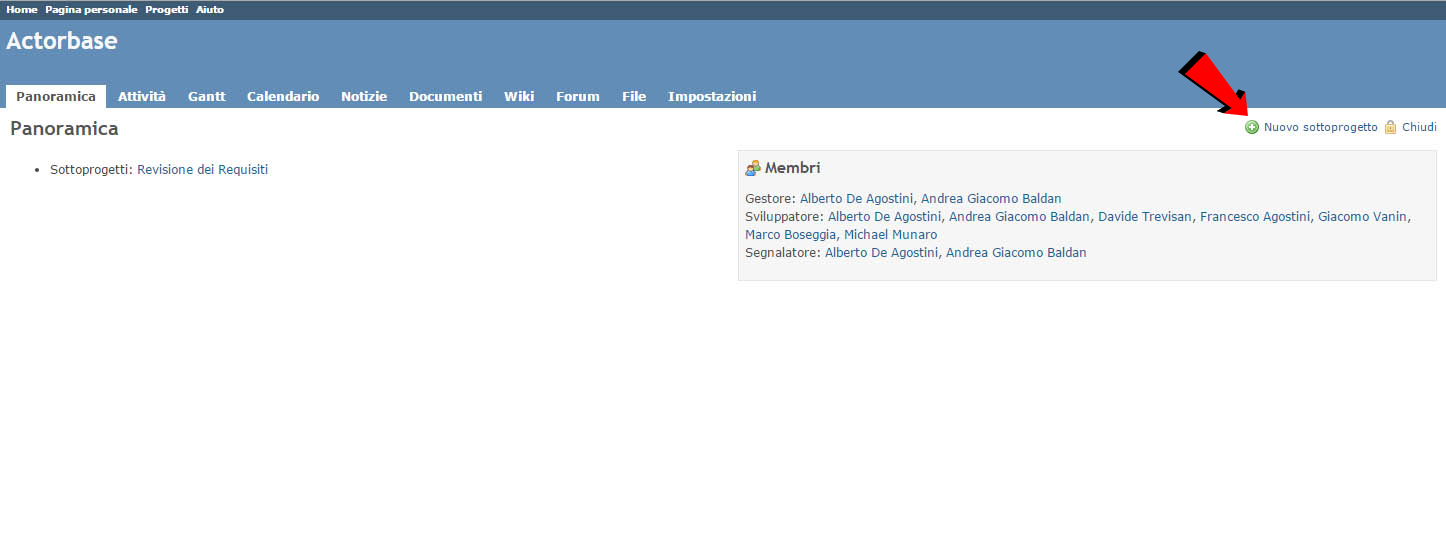
\includegraphics[width=1\textwidth]{tutorialsRedmine/creaproj1.png}
  \caption{come creare un sottoprogetto\ -\ passo 1}
\end{figure}
\begin{figure}[H]
  \centering
  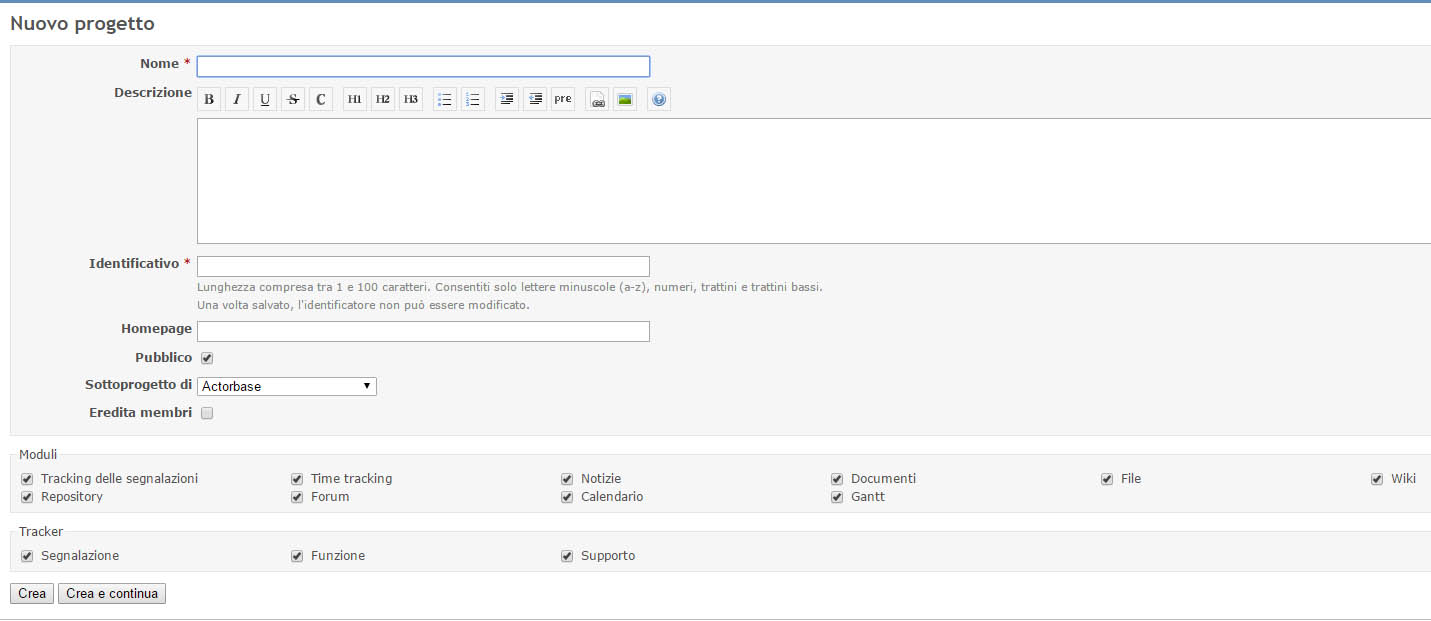
\includegraphics[width=1\textwidth]{tutorialsRedmine/creaproj2.jpg}
  \caption{come creare un sottoprogetto\ -\ passo 2\label{fig:figura-2}}
\end{figure}
Come si può vedere in figura~\ref{fig:figura-2} si dovrà completare un \gloss{form} con i dati necessari per la creazione del progetto.

\subsection{Scrivere sul Forum}

Si può partecipare al \gloss{forum} rispondendo a messaggi o creandone di nuovi

\subsubsection{Creare un messaggio}

Per creare un nuovo messaggio basta andare nel \gloss{topic} desiderato e seguire la procedura come illustrato nelle seguenti immagini
\begin{figure}[H]
  \centering
  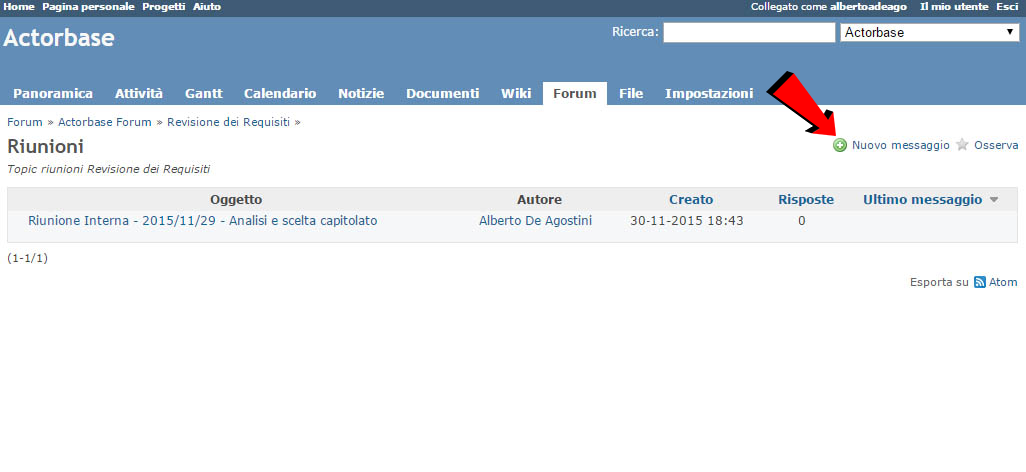
\includegraphics[width=1\textwidth]{tutorialsRedmine/creamessaggio1.png}
  \caption{come\ creare\ un\ messaggio\ -\ passo\ 1}
\end{figure}
\begin{figure}[H]
  \centering
  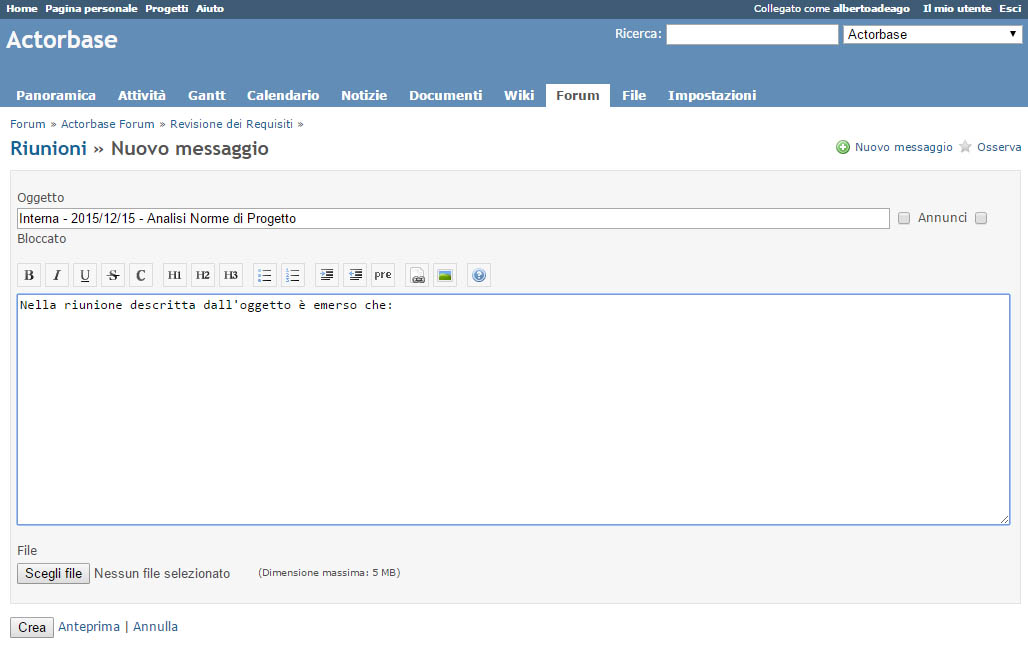
\includegraphics[width=1\textwidth]{tutorialsRedmine/creamessaggio2.jpg}
  \caption{come\ creare\ un\ messaggio\ -\ passo 2}
\end{figure}
Per la corretta creazione di un messaggio è necessario seguire le norme scritte nella sezione~\ref{sec:ComunicazioniInterne}

\subsubsection{Rispondere ad un messaggio}

Per rispondere ad un messaggio presente nel \gloss{forum} è necessario aprire il messaggio desiderato e clickare su \textbf{Rispondi}. Automaticamente si presenterà un \gloss{form} \textit{pre compilato} in cui sarà necessario solamente inserire il corpo della nostra risposta.

\subsection{Gestione delle segnalazioni}

Una segnalazione rappresenterà una \gloss{attività} che il \textit{Responsabile} assegnerà ad uno o più membri del gruppo. Queste \gloss{attività} possono essere suddivise in diversi compiti più semplici da assegnare ad un membro; quest'ultimi saranno chiamati \gloss{task}.\\
Il sistema di segnalazioni è la cosa più importante di \textit{Redmine}, perciò solamente il \textit{Responsabile di Progetto} ha il potere di creare nuove segnalazioni così da mantenere ordine nel progetto. \\Gli altri membri del gruppo potranno invece aggiornare le segnalazioni a loro assegnate.

\subsubsection{Creare una segnalazione}

Il \textit{Responsabile di Progetto} può creare nuove segnalazioni come illustrato nelle seguenti immagini
\begin{figure}[H]
  \centering
  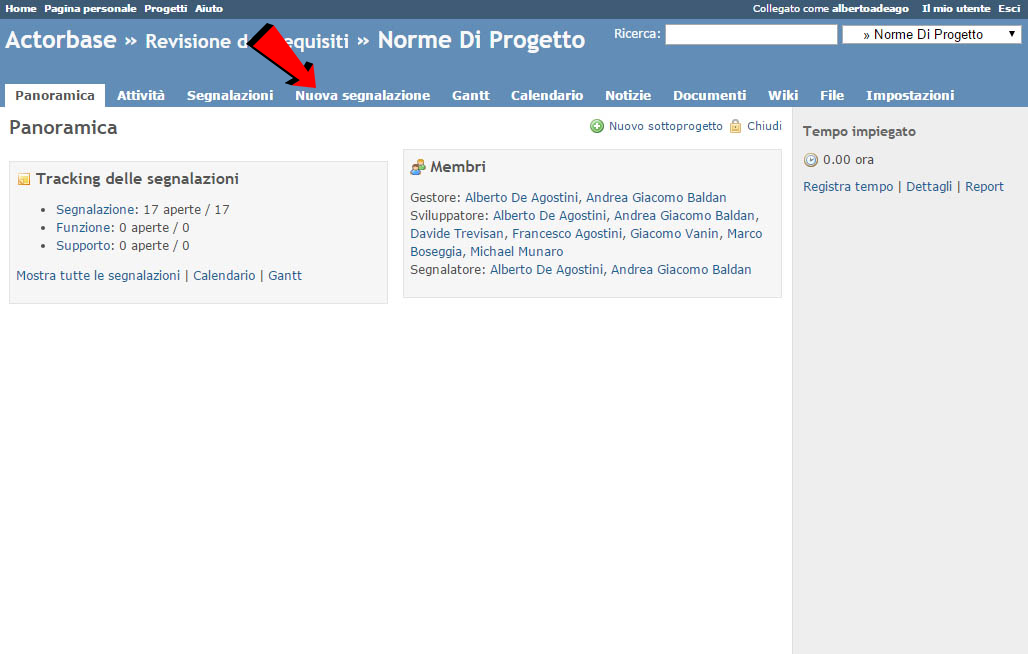
\includegraphics[width=1\textwidth]{tutorialsRedmine/creasegn1.png}
  \caption{come\ creare\ un\ segnalazione\ -\ passo\ 1}
\end{figure}
\begin{figure}[H]
  \centering
  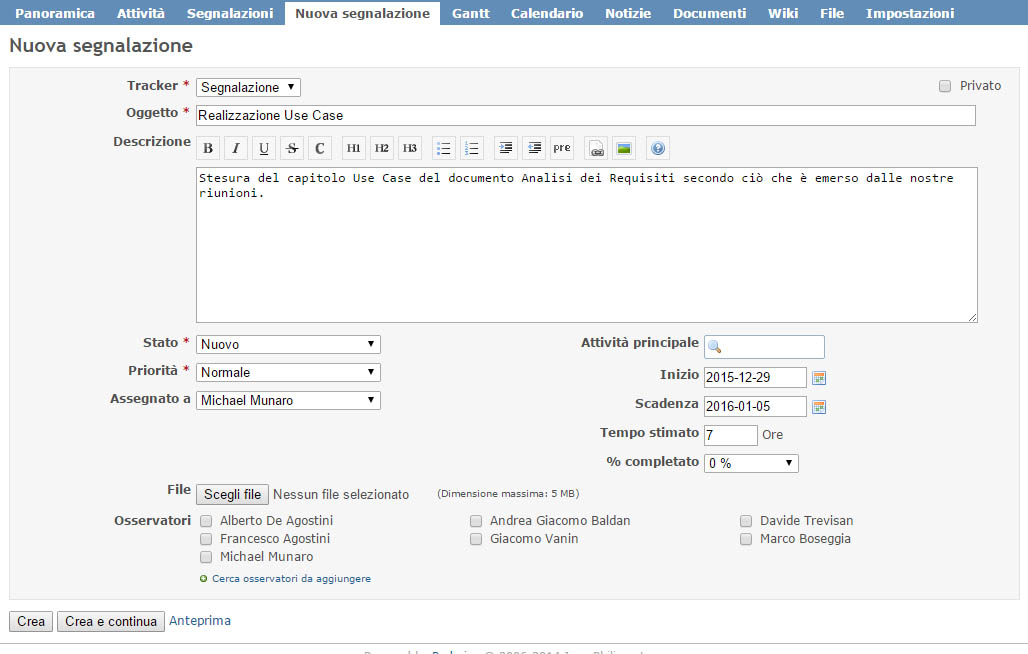
\includegraphics[width=1\textwidth]{tutorialsRedmine/creasegn2.jpg}
  \caption{come\ creare\ una\ segnalazione\ -\ passo\ 2\label{fig:crea-segnalazione-2}}
\end{figure}
Dalla figura~\ref{fig:crea-segnalazione-2} è possibile notare diversi campi da compilare:
\begin{itemize}
\item \textbf{Tracker:} lasciare selezionato \textit{Segnalazione};
\item \textbf{Oggetto:} l'oggetto della segnalazione, questo deve essere breve e non equivocabile;
\item \textbf{Descrizione:} descrizione dettagliata dell'\gloss{attività} da svolgere;
\item \textbf{Stato:} se è una nuova segnalazione deve rimanere \textit{nuovo}, altrimenti è possibile scegliere altre opzioni; lo stato viene cambiato dall'intestatario della segnalazione stessa;
\item \textbf{Assegnato a:} la persona che deve svolgere l'\gloss{attività};
\item \textbf{\gloss{Attività} principale:} se si tratta di un sotto \gloss{task} di un'altra attività, bisogna inserire l'identificatore del \gloss{task} padre;
\item \textbf{Inizio:} data in cui deve iniziare l'\gloss{attività};
\item \textbf{Fine:} data entro cui l'\gloss{attività} deve essere completata;
\item \textbf{Tempo stimato:} il numero di ore stimato entro cui si dovrebbe completare l'\gloss{attività};
\item \textbf{\% completato:} la percentuale di completamento dell'\gloss{attività}; anche questo parametro viene utilizzato dal membro del gruppo che lavora sull'\gloss{attività}.
\end{itemize}

\subsubsection{Aggiornare una segnalazione}

Il lavoro di aggiornamento di una segnalazione deve essere svolto dai vari
membri del gruppo che lavorano alla segnalazione stessa.\\ Ad ogni avanzamento
relativo ad una \gloss{attività} si deve aggiornare la segnalazione relativa ad
essa. Per fare ciò bisogna entrare nella pagina personale di \textit{Redmine} e,
nella sezione \textbf{Le mie segnalazioni}, selezionare la segnalazione
desiderata, quindi premere su \textbf{Modifica}. La schermata che si presenterà
davanti permetterà diverse operazioni come mostrato in figura~\ref{fig:crea-segnalazione-2},
si dovrà quindi aggiornare lo \textbf{stato} (se
cambiato), la \textbf{\% completata} e aggiornare inoltre il \textbf{tempo
  impiegato}. Vi è inoltre la possibilità di inserire un testo libero; questo
può essere utile per spiegare i cambiamenti apportati.

\subsection{Modificare la Wiki}

La nostra scelta è stata di usarla come raccoglitore di \gloss{link} a guide inerenti al nostro progetto.
Per contribuire alla \gloss{Wiki} basta andare nella suddetta sezione e premere su \textbf{modifica}. Si presenterà un editor di testo in cui è possibile modificare o semplicemente aggiungere del testo.

\subsection{Aggiungere impegni al calendario}

Ogni collaboratore presente su Redmine ha la possibilità di aggiungere i propri impegni sul calendario per facilitare così la suddivisione delle attività da pianificare da parte del \textit{Responsabile}.\\
Ognuno è invitato a inserire i propri impegni su questo calendario il prima possibile per agevolare il lavoro di pianificazione.

\listoffigures

\end{document}
